\documentclass[a4paper, 10pt] {article}
\usepackage{graphicx}
\usepackage{fancyhdr}
\usepackage[parfill]{}

\pagestyle{fancyplain}
%
% Title
%
\title {CLIgen Manual\\ {\small CLIgen version 4.5}}

\author{Olof Hagsand}
%
% Go!
%

\begin{document}

% If you want a logo
% \lhead{\includegraphics[height=9mm]{../../doc/logga_crop.png}}
\date{Oct, 2020}
\maketitle
\setcounter{tocdepth}{2}
\tableofcontents
\newpage
\section{Introduction}
\label{sec:intro}

CLIgen builds interactive syntax-driven \emph{command-line interfaces}
in C from a high-level syntax specification. Interactive CLIs are
often used in communication devices such as routers and
switches. However, any devices with a textual, syntax-driven,
command-based interface can use CLIgen to make CLI programming easy.

CLIgen takes a syntax specification as input, generates a tree
representation of the syntax, and provides an interactive command-line
tool with completion, help, modes, etc.

A designer formulates the command-line syntax and writes callback
functions in C to implement the semantics of the commands.

A good starting point is the hello world example with a simple syntax
specification ("hello world") and a callback with a print statement,
which produces the following CLI executable:

\begin{verbatim}
  > ./cligen_hello 
  hello> hello world 
  Hello World!
  hello> 
\end{verbatim}

The complete {\tt cligen\_hello} C application is included in the
source code distribution.

\begin{figure}
\centering
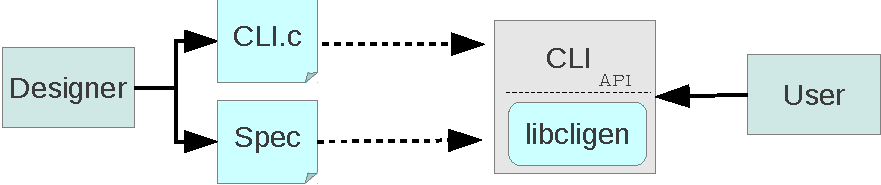
\includegraphics[scale=0.8]{usage.pdf}
\caption{\em CLIgen usage: a designer implements a CLI by specificying the syntax in a specification file and the CLI source code using the CLIgen API.}
\label{fig:usage}
\end{figure}

Figure~\ref{fig:usage} shows a typical workflow when working with
CLIgen. A designer specifies the CLI syntax by editing a CLIgen
specification file and writing a C-program. When users access the CLI
at runtime, the specification file is loaded and the CLI uses the API
of the CLIgen library to interpret the commands.

An example of a CLIgen specification file of the hello world application is:
\begin{verbatim}
  prompt="hello> "             # Assignment of prompt
  hello("Greet the world"){    # 'hello' command with help text
    world, cb("Hello World!"); # 'world' command with callback
  }
\end{verbatim}

The specification above shows examples of the following key ingredients of a specification:
\begin{itemize} 
\item
\emph{Command syntax} specifies the syntax of the actual commands, and
are the main part of a specification. The command syntax is fully
described in Section~\ref{sec:syntax}.
\item
\emph{Callbacks} are functions called when a command has been entered
by a user. You may specify an argument to a callback. Callbacks
are a part of the API described in Section~\ref{sec:api}.
\item
\emph{Assignments} are used to set properties of the CLI and its
commands, such as prompts, visibility, etc. Assignments are either global or per-command.
\item
\emph{Help text} provides help text for individual commands.
\item
\emph{Comments} begin with the '\#' sign.
\end{itemize}

The following sections will describe all aspects of designing CLIgen
application. Programming using the CLIgen API in C is described in
Section~\ref{sec:api}.

\section{Command syntax}
\label{sec:syntax}

The command syntax consists of a combination of keywords, variables and
operators:
\begin{itemize}
\item
\emph{Keywords} are constant strings representing fixed command words.
\item
\emph{Variables} are placeholders for user-defined input.
\item
\emph{Operators} are used to combine keywords and variables in different ways. Operators
include 'choice', 'option', 'sequence', etc. Operators are further described in Section~\ref{sec:operators}.
\end{itemize}

For example, the command syntax {\tt ip tcp <uint16>;} have two keywords:
{\tt ip}, and {\tt tcp} and one variable: {\tt <uint16>}. They are
combined in a \emph{sequence}, that is, the CLI expects them to be
typed one after the other.

\subsection{Keywords}

The simplest syntax consists only of keywords. Such a syntax can be
specified as follows:
\begin{verbatim}
  aa bb{
    ca;
    cb;{
      dd;
      ee;
    }
  }
  ff;
\end{verbatim}
A CLI loaded with the specification above accepts the following strings as input:
\begin{verbatim}
  aa bb ca
  aa bb cb
  aa bb cb dd
  aa bb cb ee
  ff
\end{verbatim}
Note the following:
\begin{itemize}

\item Newlines are not significant, except after comments. This means
  that another way of specifying the syntax above is: {\tt aa
    bb\{ca;cb;\{dd;ee;\}\}ff;}.

\item Keywords specified one after another is a
  sequence. Example: {\tt aa bb;}. An alternative of expressing the same syntax is: {\tt aa\{bb;\}}

\item Semicolon terminates a complete command. This means that {\tt aa bb cb}
 is accepted as a complete command, but not {\tt aa bb} in the syntax above.

\item Semicolons also act as a choice, you can choose either {\tt dd}
  or {\tt ee} in the syntax above.

\item Keywords can also be specified using variables: {\tt
  <string keyword:aa>}, there are some advantages with this which may
  get apparent when programming using the API (see
  Section~\ref{sec:api}).

\item The syntax above can be written in a more compact way, such as {\tt aa bb (ca|cb [dd|ee]);ff;}. This is described more in Section~\ref{sec:operators}

\end{itemize}

\subsection{Runtime behaviour}

A CLI with the syntax above will present the user with a list of
commands. On the top-level, only {\tt aa} or {\tt bb} may be chosen when a question mark is entered:
\begin{verbatim}
  > '?'
    aa
    gg
\end{verbatim}

If the user prints an 'a', followed by a 'TAB', the CLI performs
completion to {\tt aa} since there is only one alternative:
\begin{verbatim}
  > a'TAB'
  > aa 'TAB'
  > aa bb 'TAB'
  > aa bb c'TAB'
  ca                  cb
  > aa bb c
\end{verbatim}
In the example, two more {\tt TAB}s are entered, one for each command
level and completion continues until the commands are not unique. In
the last {\tt TAB}, the CLI shows the available commands ({\tt ca} and {\tt cb}).

As long as a command is unique it is not necessary to
complete the whole string. For example, the following two strings are
equivalent from the CLIs perspective:
\begin{verbatim}
  > aa bb cb dd
  > a b cb d
\end{verbatim}

Before finishing a command (with return), a unique
command must be selected. The CLI gives an error code if the command
is unknown, ambiguous or incomplete:
\begin{verbatim}
> a
CLI syntax error in: "a": Incomplete command
> aa bb c
CLI syntax error in: "aa bb c": Ambiguous command
> aa bb dd
CLI syntax error in: "aa bb dd": Unknown command
\end{verbatim}

\subsection{Escaping}

In the CLIgen runtime, some characters have special meaning, such as
{\tt '?'}. You can \emph{escape} characters with backslash({\tt '\textbackslash'}) so
that for example {\tt '?'} can appear in a keyword or value:
\begin{verbatim}
> a\?b # Gives the string "a?b"
> a\\b # Gives the string "a\b"
\end{verbatim}

\subsection{Help texts}

Help texts are given within parenthesis following a keyword or
variable. The help text appears when you invoke the help command '?'
in the CLI runtime.

For example, assume the following syntax:
\begin{verbatim}
  ip("The IP protocol"){
    udp("The UDP protocol") <ipaddr>("IPv4 address");
    tcp("The TCP protocol") <uint16>("Port number");
  }
\end{verbatim}
If a user has typed 'ip ' and '?', the following help text appears:
\begin{verbatim}
cli> ip '?'
  tcp                      The TCP protocol
  udp                      The UDP protocol
\end{verbatim}

\subsection{Callbacks}
\label{sec:callbacks}

When a unique command has been selected, a callback may be
called. Callbacks are typically associated with commands using the
file syntax:
\begin{verbatim}
  aa bb{
    ca,fn1("ca");
    cb,fn1("cb");{
      dd,fn2();
      ee,fn3((int)42);
    }
  }
\end{verbatim}

In the example, the function {\tt fn1} is called with {\tt "ca"} as
argument if {\tt aa bb ca}, is selected. The same function is called
also if {\tt aa bb cb} is selected, but with another argument. For
other commands, {\tt fn2} is called without argument, and {\tt fn3} is
called with the integer argument {\tt 42}.

Note that callbacks may only be associated with terminal commands. For
example, {\tt aa bb} may not have a callback function.

The details on how to write callback functions, such as {\tt fn1} -
{\tt fn3} is described in detail in Section~\ref{sec:api}.

\subsection{Assignments}
\label{sec:assignments}

You can assign values to \emph{global} and \emph{local}
variables. Global variables are valid for the whole syntax, while
local variables only apply to a single command.

In the current release, there is one pre-defined local variable: 
\begin{itemize}
\item
{\tt hide} specifies that a command is not visible when listing or
completing commands with '?' and 'TAB'.  Still, the command is
selectable and may be selected if you type it. This can be useful if there are
commands that should be known only by expert users.
\end{itemize}

In the following example, {\tt aa bb cb dd} and {\tt aa bb cc} are not visible:
\begin{verbatim}
  aa bb{
    ca;
    cb,hide{
      dd;
    }
    cc,hide;
  }
\end{verbatim}

A {\em global} variable is assigned on the top-level.  There is
currently only one pre-defined global variable ({\tt treename} as
described in the next section).  But it is easy for a programmer to
implement a global variable and define semantics to it. 

The tutorial application supports prompt and comment character:
\begin{verbatim}
  prompt="cli> ";              # Assignment of prompt
  comment="#";                 # Same comment as in syntax
\end{verbatim}
Section~\ref{sec:global} describes how the C-API can be used to define
semantics for a global variable.

\subsection{Trees}

CLIgen can handle multiple syntax trees. A user can switch between
trees (i.e., change CLI mode), or extend a tree with a sub-tree (using
tree-references). 

A tree is named using a special global {\tt treename} assignment. The
following example shows two syntax trees: {\tt tree1} and {\tt tree2}.
\begin{verbatim}
  treename="tree1";
    x{
      y;
    }
  treename="tree2";
    z{
      x;
    }
\end{verbatim}

When parsing the syntax above, a CLIgen tree-list consisting of two
trees will be created. By default, the first parsed tree is the active tree.

\begin{verbatim}
 changetree <tree:string>, changetree("tree2");
\end{verbatim}

Note that the {\tt changetree} callback needs to be implemented as a
callback function in C to actually change the syntax mode. Such a
callback is implemented in the tutorial and is also described in more
detail in Section~\ref{sec:api}.

Note, the {\tt treename} feature is not available in Clixon, only in stand-alone CLIgen.

\subsubsection{Tree references}

A CLIgen syntax tree may reference another tree as an extension using
the reference operator '@'.

The following specification references itself:
\begin{verbatim}
  treename="T";
  foo;
  recurse @T;
\end{verbatim}
which means that the following sentences are valid commands:
\begin{verbatim}
  foo
  recurse foo
  recurse recurse foo
  recurse recurse recurse foo
\end{verbatim}
and so on.

Callbacks can be parametrized when using tree references. This means
that you can specify which callback to use in the reference of the
tree. This means that different callbacks can be called depending on
how you reference the tree.

The following examples shows a main tree and a sub-tree. 

\begin{verbatim}
  treename="main";
  add @sub, add();
  del @sub, del();
  treename="sub";
  x{
    y, fn("a");
  }
\end{verbatim}

% (1) funktionen fr�n anropet anv�nds alltid, dvs fn i @sub,fn(arg)
% (2) Om det finns en funktion i ur-tr�det, s� anv�nds dess parameter-lista. Dvs arg i fn(arg).
% (3) Om det inte finns en funktion i ur-tr�det, s� anv�nds b�de funktionen och argument-listan fr�n anropet, dvs fn(arg) i @sub,fn(arg)

The main tree references the subtree twice. In the first reference,
{\tt add("a")} is called when invoking the command {\tt add x y}. In the
second instance {\tt del("a")} is invoked when invoking the command {\tt del x y}.

Note that the parameter list {\tt ("a")} is not substituted, the original is
used. In the example this means that {\tt add("a")} is called
regardless of any parameters to {\tt add()} in the {\tt @sub}
invocation. An exception to this rule if there is no callback given in
the original tree (e.g. as in {\tt x \{ y; \}}, then the callback and argument
list from the tree reference is used (eg add() including aventual
parameter list)\footnote{Yes, this semantics is somewhat complex and
  needs revision}.

It may be useful with functional substitution as shown above when the
subtree represents a large common data-modeling sub-tree, where the
data (x y) is the same but the operation(add/del) is different.

In the example, the 'treename' variable is used to define a new CLIgen
tree. It is possible using the C-API to change this keyword to
something else by using the API function {\tt cligen\_treename\_keyword}.

\subsubsection{Tree workpoints}

When using tree references it is possible to set an active {\em
  workpoint} for that tree, which can change dynamically. In this way,
a user can navigate up and down the tree in its references for it. This
is useful when implementing automatic modes for example.

To achieve this, a couple of C-API callbacks are available:
\begin{itemize}
  \item {\tt cligen\_wp\_set(<tree>)} - Set the workpoint
  \item {\tt cligen\_wp\_show(<tree>)} - Show the tree at the active workpoint
  \item {\tt cligen\_wp\_up(<tree>)} - Navigate up in the tree
  \item {\tt cligen\_wp\_top(<tree>)} - Navigate to top of tree
\end{itemize}

Assume first a tree ``T'' is created that will be navigated in using workpoints:
\begin{verbatim}
     treename="T";
     a; {
       b <v:int32>; {
         d;
       }
       c;
     }
\end{verbatim}

Then, some main syntax for navigating in three is added in the main CLIgen spec:

\begin{verbatim}
  edit, cligen_wp_set("T");{
    @T, cligen_wp_set("T");
  }
  show, cligen_wp_show("T");
  up, cligen_wp_up("T");
  top, cligen_wp_top("T");
\end{verbatim}

It is now possible to traverse the tree using the ``T'' tree as the following example illustrates (the prompt shows the location of the active workpoint):
\begin{verbatim}
     cli:/> show 
     a;{
        b <v>;{
              d;
           }
        c;
     }
     cli:/> edit a 
     cli:/a> show 
     b <v>;{
           d;
        }
     c;
     cli:/a> edit b 23
     cli:/a/b/23> show 
     d;
     cli:/a/b/23> up
     cli:/a/b> show 
     <v>;{
        d;
     }
     cli> top
     cli:/> show 
     a;{
        b <v>;{
              d;
           }
        c;
     }
     cli:/> 
\end{verbatim}

\subsection{Sets}

By default, listing several commands within {\tt \{\}} gives a choice of commands, but if instead commands are within the set operator {\tt @\{\}}, the commands can be given on any order, and at least once. For example:
\begin{verbatim}
  x @{
    a;
    b;
    c;
  }
\end{verbatim}

gives exactly the following allowed CLI commands, and no others:
\begin{verbatim}
  x a
  x a b
  x a b c
  x a c
  x a c b
  x b
  x b a
  x b a c
  x b c
  x b c a
  x c
  x c a
  x c a b
  x c b
  x c b a
\end{verbatim}

Note that the sets implementation is EXPERIMENTAL in the current release, and you may need to define the {\tt USE\_SETS} option in {\tt cligen\_custom.h}.

\section{Variables}
\label{sec:variables}
Variables are placeholders for user input. They also give support for
lexical checking. The {\tt int32} type, for example, only
accepts 32-bit integers, while {\tt string} accepts any sequence of
characters. 

\subsection{Basic structure}

A variable has the following basic components:
\begin{itemize}
\item {\em name} - How the variable is referenced, such as in a callback.
\item {\em type} - The type of the variable. If no type is given, it is by default the same as {\em name}.
\item {\em show} - How the variable is displayed in help texts (such as after a '?' or 'TAB'. If no show field is given,  it defaults to {\em name}.
\end{itemize}

The variable syntax has several forms:
\begin{verbatim}
  <int32>;                
  <a:int32>;              
  <a:int32 show:"a number">("A 32-bit number")
\end{verbatim}

In the first form, both name, type and show is {\tt int32}. In the
second form, the name and show is "a", while type is {\tt int32}. 
In the last form, all fields are explicitly given, and there is also a help-text.

An example of the last, most explicit form in a CLI:
\begin{verbatim}
  cli> '?'
     <a number>        A 32-bit number
\end{verbatim}

\subsection{String}
The simplest form of a string specification is: {\tt
<string>}, which defines a string variable with the name 'string'.

A more advanced string variable specification is the following:
\begin{verbatim}
  address <addr:string>("Address to home");
\end{verbatim}
where the name of the string variable is {\tt addr}. The name can be used when referring to the variable in a callback, and is also used in the help text:
\begin{verbatim}
  cli> address '?'
     addr          Address to home
\end{verbatim}

A string may contain all characters with some minor exceptions. Most
notably, a string can not contain a question mark, since it is used
for querying syntax in the CLI.  Also, if a string contains spaces, it
must be contained within double quotes.  The following examples are all valid
strings:
\begin{verbatim}
  i_am_a_string
  ()/&#
  "I am a string"
  ab"d
\end{verbatim}

A string can be constrained by a {\tt length} statement. If given, the number of characters in a string is limited to a min/max interval, or just a max\footnote{Note that this differs from YANG types where a single bound means exactly that value, see RFC 7950}.

Example:
\begin{verbatim}
  <addr:string length[8:12]>
  <addr:string length[12]>
  <addr:string length[2:4] length[8:12]>
\end{verbatim}
which means that the {\tt addr} string, if given, must be between 8 and 12 characters long, or just limited to 12 characters, or be between 2-4 and 8-12 charcters respectively.

A variant of string is {\tt rest} which accepts all characters until
the end-of-line. 


\subsection{Integers}
There are several integer variables, signed, unsigned, and 8, 16, 32 or 64-bits. For example, the {\tt int32} variable allows any 32-bit integer, and can be specified in decimal or hex format. 

Further, an allowed range of integer can specified, either as an interval or as an upper limit, or a set of ranges:

Examples:
\begin{verbatim}
  <x:uint32>
  <x:int8 range[-12:80] range[100:110]>>
  <x:int64 range[1000]>
\end{verbatim}

\subsection{Addresses}

CLIgen is often used in communication devices. Therefore, there is
support for several pre-defined address types.  Special lexical
checking is defined for those types:

\begin{itemize}
\item {\tt ipv4addr} - An IPv4 address in dotted decimal notation. Example: {\tt 1.2.3.4}
\item {\tt ipv4prefix} - An IPv4 prefix in 'slash' notation: Example: {\tt 1.2.3.0/24}
\item {\tt ipv6addr} - An IPv6 address. Example: {\tt 2001::56}
\item {\tt ipv6prefix} - An IPv6 prefix. Example: {\tt 2001:647::/64}
\item {\tt macaddr} - A MAC address: Example: {\tt 00:E0:81:B4:40:7A}
\item {\tt url} - An URL: Example: {\tt http://www.hagsand.se/cligen}
\end{itemize}

CLIgen performs lexical checking of the address variables, an invalid
address is considered as a syntax error.

\subsection{Uuid}

A variable of type {\tt uuid} accepts uuid according to standard syntax,
such as {\tt f47ac10b-58cc-4372-a567-0e02b2c3d479}. 


\subsection{Time}

A {\tt time} variable accepts ISO timestamps on the form

\begin{verbatim}
  2008-09-21T18:57:21.003456
  2008-09-21 18:57:21.003456
  2008-09-21 18:57:21
\end{verbatim}

\subsection{Boolean}

A variable of {\tt bool} type accepts the values {\tt true}, {\tt
  false}, {\tt on} and {\tt off}.

\subsection{Decimal64}

A variable of type {\tt decimal64} defines a subset of floating point
numbers that can be obtained by multiplying a 64-bit signed integer
with a negative power of ten, ie as can be expressed by $i * 10^{-n}$,
where $n$ is between 1 and 18.

The number of fraction-digits can be defined in the specification of
the type, if this is not defined explicitly, the default number of decimals is 2.

Two examples of decimal64 are {\tt 732848324.2367} (four
fraction-digits) and -23.0 (one fraction-digit).

Examples of decimal64 specification is:
\begin{verbatim}
  <d:decimal64 fraction-digits:4>;
  <d:decimal64 fraction-digits:4 range[0.1:10]>;
\end{verbatim}
which allows numbers with four decimals. The econd example limits the numbers to be between 0.1000 and 10.0000.

Note that the {\tt fraction-digits} statement should come before the {\tt range} statement.

\subsection{Keyword}
\label{sec:keyword}

A keyword variable is just an alternative way of specifying command
keywords as defined in Section~\ref{sec:syntax}. In fact, a syntax
with static keywords can just as well be written using keyword
variables. 

Thus, for example, the two specification lines below are equivalent:
\begin{verbatim}
  aa bb;
  <aa:string keyword:aa> <bb:string keyword:bb>;
\end{verbatim}

However, a keyword variable can have another name:
\begin{verbatim}
  <myname:string keyword:aa>;
\end{verbatim}

Naming of keywords provides for more flexible search functions
in callbacks, see Section~\ref{sec:api}.

Note that a keyword must be of type {\tt string}.

\subsection{Choice}

The choice variable can take the value from a static list of elements.

Example:
\begin{verbatim}
  interface <ifname:string choice:eth0|eth1>("Interface name");
\end{verbatim}

A CLI user will get the following choice:
\begin{verbatim}
  cli> interface '?'
     eth0        Interface name
     eth1        Interface name
  cli> 
\end{verbatim}
The user can only select eth0 or eth1, and thus the value of the {\tt
  ifname} variable is either {\tt eth0} or {\tt eth1}.

Note the resemblance with choice of strings in
Section~\ref{sec:operators} where the same example could be specified
as:
\begin{verbatim}
  interface (eth0|eth1)
\end{verbatim}

Again, the former variant allows for naming of the variable which can
be better when writing a callback function. In the example, the name
of the variable in the first example is {\tt ifname} whereas in the
second it is \emph{either} {\tt eth0} or {\tt eth1}.

\subsection{Expand}
\label{sec:expand1}
The choice variable specifies a static list of
keywords. But what if the list is dynamic and changes over time?

The expansion variable is a \emph{dynamic} list of keywords, where the
list may be different each time the CLI command is invoked.

For example, assume a user can select a network interface in the CLI,
but the number of interfaces changes all the time. This can be
specified as follows:

\begin{verbatim}
  interface <ifname:string interfaces()>("Interface name")
\end{verbatim}
The user's choice in the CLI will then be just as in the choice case:
\begin{verbatim}
  cli> interface '?'
     eth0        Interface name
     eth1        Interface name
  cli> 
\end{verbatim}

However, at another point in time, the choice of interfaces may be different:
\begin{verbatim}
  cli> interface '?'
     eth3        Interface name
     lo0         Interface name
  cli> 
\end{verbatim}

There is one catch here: the CLI needs to know in run-time the members
of the list. That is, the list members cannot be specified in the
syntax.  In CLIgen, the application programmer defines a C callback
function, {\tt interfaces()} in this example, which computes the list
at the time it is needed. This callback is registered and called
whenever necessary.

How to write an expand callback is further described in
Section~\ref{sec:expand}.

\subsection{Regular expressions}

A string variable may be described using a regular expression. That
is, a regular expression defines which values are valid. 

For example, a variable may be specified as:
\begin{verbatim}
  <name:string regexp:"(ab|a)b*c">;
  <name:string regexp:"[a-z]+[0-8]+\\.[0-9]">;
\end{verbatim}
The first rule matches the following strings, for example:
\begin{verbatim}
ac
abc
abbbbbbbbbc
\end{verbatim}

You can also add multiple regexps, in which case the string must match ALL regexps. You can also specify an inverted regex, meaning that a string should NOT match the regex.

In the following example, all strings are matched that do not start with "cli"
\begin{verbatim}
    <name:string regexp:"[a-zA-Z]+" regexp:!"cli.*">;
\end{verbatim}

CLIgen by default uses POSIX Extended regular expression syntax.
However, XML schema regexps can be used instead by configuring CLIgen with libxml2 as follows:
\begin{verbatim}
   ./configure --with-libxml2     # At configure time
   cligen_regexp_xsd\_set(h, 1);  # In C init code
\end{verbatim}

\subsection{Variable translation}

CLIgen supports variable translation. A given variable can be
translated on-th-fly using a generic translation function. This may be useful for example when hashing or encrypting a value.

In the example below, the variable {\tt var} is translated by the function {\tt incstr}:
\begin{verbatim}
    increment <var:string translate:incstr()>, cb();
\end{verbatim}

In this example, {\tt incstr} simply increments every character in the variable.
\begin{verbatim}
    cli> increment HAL
    variables:        1 name:var type:string value:IBM
\end{verbatim}

In the same way, a clear text password could be translated to an encrypted string.
For information on how to implement a translator function, see Section~\ref{sec:translate}.

\section{Operators}
\label{sec:operators}

In the regular syntax format, there are (implicit) sequence and choices. For example, the syntax
\begin{verbatim}
  aa bb;
  cc;
\end{verbatim}
defines a choice between the sequence {\tt aa bb} and {\tt cc}.

It is also possible to explicitly define choices, optional elements and syntactical groupings.


\subsection{Choice and grouping}
Explit choice between several elements can be made as follows:
\begin{verbatim}
  (aa bb) | cc;
\end{verbatim}
which expresses the same syntax as above.

Help strings work as usual, but may \emph{not} be associated with
groupings:
\begin{verbatim}
  aa (bb("help b") cc("help c") | dd("help d"));
\end{verbatim}

Choices may also be made with variables:
\begin{verbatim}
  values (<int8> | <string> | <int64> | aa);
\end{verbatim}

where a pattern matching is made selecting to try to select the most 'specific'
variable. For example, the following input will give different matchings:
\begin{itemize}
\item
{\tt aa} selects the keyword.
\item
{\tt bb} selects {\tt <string>}.
\item
{\tt 42} selects {\tt <int8>}.
\item
{\tt 324683276487326} selects {\tt <int64>}.
\end{itemize} 

\subsection{Optional elements}
It is also possible to express an \emph{optional} part of a syntax
using brackets:
\begin{verbatim}
  aa [[bb] cc];
\end{verbatim}
which accepts the commands: {\tt aa}, {\tt aa bb} and  {\tt aa bb cc}.

Any combination of these operations are possible, such as in the line:
\begin{verbatim}
  aa [[(bb|cc <int32>)] dd] ee;
\end{verbatim}

Note that the elaborate command specifications above can be combined
in a regular syntax, at parsing they are just expanded into a larger
syntax tree. 
Thus for example, the syntax:
\begin{verbatim}
  aa bb (ca("help ca")|cb("help cb")) [dd|ee];
\end{verbatim}
is equivalent to:
\begin{verbatim}
aa bb{
   ca("help ca");{
      dd;
      ee;
   }
   cb("help cb");{
      dd;
      ee;
   }
}
\end{verbatim}
which is similar to the syntax used in Section~\ref{sec:syntax}.


\subsection{Caveat}

Note that the choice, groupings and optional elements are only
syntactical structures generating the basic constructs described
earlier. This means that if you use too many of them, they can
generate a large number of states and consume memory.

For example, the optional operator {\tt []} will increase the number of states with a
factor of two. Thus {\tt [a][b][c][d]} will generate 16 states, for
example.

As an assistant, you can use the {\tt -p} option to {\tt cligen\_file} to see which basic syntax is generated:
\begin{verbatim}
   $ echo "[a][b][c];" | ./cligen_file -p
   a;{
      b;{
         c;
      }
      c;
   }
   b;{
      c;
   }
   c;
\end{verbatim}

\section{API}
\label{sec:api}
This section describes C-programming issues, including types, parsing and
callbacks.

Appendix A contains a complete program illustrating many of the topics
of this tutorial.  More advanced applications can be found in the CLIgen
source repository.

\subsection{CLIgen variables}

Variables in the command syntax (such as {\tt <string>}) described in
Sections~\ref{sec:variables} and \ref{sec:assignments} are translated
in runtime into \emph{CLIgen variables} using the {\tt cg\_var}
datatype.  A CLIgen variables is sometimes referred to as a \emph{cv}.

A cv is a handle and its values are accessed using get/set
accessors. Two generic fields are {\tt name} and {\tt type}, other
fields are accessed via type-specific accessors (see next Section).

Example: get name and type of cligen variable:
\begin{verbatim}
  char *name        = cv_name_get(cv);
  enum cv_type type = cv_type_get(cv);
\end{verbatim}


\subsubsection{Types}

CLIgen variables have a simple type-system, essentially following the
types introduced in Section~\ref{sec:variables}. Each cv type
have get/set operators to access and modify the value.

For example, a command syntax contains {\tt <addr:ipv4addr>}, and
the user inputs "12.34.56.78". The CLI will then generate a cv which
can be accessed in C. The string
"12.34.56.78" is accessed with:
\begin{verbatim}
  struct in_addr addr = cv_ipv4addr_get(cv);
\end{verbatim}

Accessors for other types are shown in the table
below. There may be several fields for a given type. These are given
in the table with the corresponding C-type.

\begin{tabular}{ | l | l | l | }
\hline
  \textbf{ Type} & \textbf{Accessor} & \textbf{C-type}\\
\hline
int8   & {\tt cv\_int8\_get()}   & {\tt int8\_t} \\
int16  & {\tt cv\_int16\_get()}  & {\tt int16\_t} \\
int32  & {\tt cv\_int32\_get()}  & {\tt int32\_t} \\
int64  & {\tt cv\_int64\_get()}  & {\tt int64\_t} \\
uint8  & {\tt cv\_uint8\_get()}  & {\tt uint8\_t} \\
uint16 & {\tt cv\_uint16\_get()} & {\tt uint16\_t} \\
uint32 & {\tt cv\_uint32\_get()} & {\tt uint32\_t} \\
uint64 & {\tt cv\_uint64\_get()} & {\tt uint64\_t} \\
decimal64 & {\tt cv\_dec64\_i\_get()} & {\tt int64\_t}\\
           & {\tt cv\_dec64\_n\_get()} & {\tt uint8\_t}\\
bool & {\tt cv\_bool\_get()} & {\tt uint8\_t} \\
string & {\tt cv\_string\_get()} & {\tt char*} \\
ipv4addr   & {\tt cv\_ipv4addr\_get()} & {\tt struct in\_addr}\\
ipv4prefix & {\tt cv\_ipv4addr\_get()} & {\tt struct in\_addr}\\
           & {\tt cv\_ipv4masklen\_get()} & {\tt uint8}\\
ipv6addr   & {\tt cv\_ipv6addr\_get()} & {\tt struct in6\_addr}\\
ipv6prefix & {\tt cv\_ipv6addr\_get()} & {\tt struct in6\_addr}\\
           & {\tt cv\_ipv6masklen\_get()} & {\tt uint8}\\
macaddr    & {\tt cv\_mac\_get()} & {\tt char[6]}\\
uuid       & {\tt cv\_uuid\_get()} & {\tt char[16]}\\
time       & {\tt cv\_time\_get()} & {\tt struct timeval}\\
url        & {\tt cv\_urlproto\_get()} & {\tt char*}\\
           & {\tt cv\_urladdr\_get()} & {\tt char*}\\
           & {\tt cv\_urlpath\_get()} & {\tt char*}\\
           & {\tt cv\_urluser\_get()} & {\tt char*}\\
           & {\tt cv\_urlpasswd\_get()} & {\tt char*}\\
\hline
\end{tabular}

You may also access a value with an unspecified type using:
\begin{verbatim}
  void *v = cv_value_get(cv);
\end{verbatim}


\subsubsection{Cligen variable vectors}
Variables are grouped into vectors whose using {\tt cvec}. Global variables or variables
passed to callback functions are always grouped into {\tt cvec}
structures.




\subsubsection{Finding variables in a vector}
\label{sec:find}



Suppose for example that you have the following command syntax:
\begin{verbatim}
person [male|female] (<age:int32>|<name:string>)
\end{verbatim}

A {\tt cvec} is accessed using a handle. Typically an iterator is used to access the individual cv:s within a vector:
\begin{verbatim}
   cvec *vr;
   cg_var *cv = NULL;
   while ((cv = cvec_each(vr, cv)) != NULL) {
      str = cv_name_get(cv);
   }
\end{verbatim}

You can also access the variables individually if you know their order, in this example the 3rd element:
\begin{verbatim}
   cvec *vr;
   cg_var *cv = cvec_i(cv, 2);
\end{verbatim}

A way to find variables using their names is as follows:
\begin{verbatim}
  cg_var *cv = cvec_find(vars, "age");
\end{verbatim}

Actually, kewords are also a part of variable vectors. This means that
they can also be accessed via their name, although the name of the
keyword is the same as its constant value, as described in
Section~\ref{sec:keyword}.

Therefore, you can also check whether a keyword exists or not. Using the same example:
\begin{verbatim}
  if (cvec_find(vars, "male") != NULL)
    printf("male\n");
\end{verbatim}
where the conditional evaluates to true only if the user has selected
{\tt male} and not {\tt female}.

\subsection{Initializing}
\label{sec:handle}

An application calls the CLIgen init function to initialize the CLIgen
library.  The function returns a {\tt handle} which is used in most
CLIgen API functions.

In the following example, CLIgen is initialized, a prompt is set, and
is then terminated:
\begin{verbatim}
  cligen_handle h = cligen_init();
  cligen_prompt_set(h, "cli> ");
  [...]
  cligen_exit(h);
\end{verbatim}

\subsection{Parsing syntax files}
\label{sec:parsing}
The command syntax as described in
Sections~\ref{sec:syntax}-\ref{sec:operators} normally resides in a
file which is loaded and parsed by the CLI. The result of the parsing
is a parse-tree and a list of global variable assignment. After
parsing, the program needs to interpret the result and set up the CLI
environment. This includes handling global variable assignments,
mapping function callbacks, etc. 

Most non-trivial programs handle many syntaxes that are merged into a
common parse-tree, while others partition parse-trees into different
modes.

An example of parsing syntax file {\tt mysyntax.cli} is the following: 
\begin{verbatim}
  cligen_handle h;
  FILE         *f;
  h = cligen_init();
  f = fopen("mysyntax.cli");
  cligen_parse_file(h, f,  "mytree", NULL, NULL);
  cligen_loop(h);
\end{verbatim}

The example code initiates a handle, opens the CLIgen syntax file, parses the
syntax into a tree called {\tt mytree} and starts a CLIgen command loop.

The next step is to handle the global variables and to bind callback
functions.

\subsection{Global variables}
\label{sec:global}

A syntax file may contain global variable assignments which can be
accessed by the the C-code. Suppose a syntax file contains the following global assignments:
\begin{verbatim}
  prompt="cli> ";              # Assignment of prompt
\end{verbatim}

These global variables are parsed and may be read by the C-code as follows:
\begin{verbatim}
  char *prompt;
  [...]
  cligen_parse_file(h, f,  "mytree", NULL, globals);
  prompt = cvec_find_str(globals, "prompt");
  cligen_prompt_set(h, prompt);
\end{verbatim}

In this way a programmer may define the semantics of global variables
by binding their value to actions.

\subsection{Command loop}
\label{sec:main}

A programmer can use the pre-defined {\tt cligen\_loop} function, or create a tailor-made loop as follows:

\begin{verbatim}
 for (;;){
     retval = cliread_eval(h, &line, &ret);
\end{verbatim}
The return value of the {\tt cliread\_eval} function is as follows:
\begin{itemize}
\item {\tt CG\_EOF}: end-of-file
\item {\tt CG\_ERROR}: CLIgen read or matching error, typically if the syntax is not well-defined.
\item {\tt CG\_NOMATCH}: No match, the input line did not match the syntax. By calling {\tt cligen\_nomatch(h)}, the reason for why no match was made is retrieved.
\item {\tt CG\_MATCH}: Match, the line matched exactly one syntactic node. The variable {\tt ret} contains the return value of the callback (if any).
\item $> 1$: Multiple matches, the line matched several syntax lines.
\end{itemize}



\section{Advanced API}

\subsection{Writing a callback function}

A programmer may write a callback function for every complete command
defined in the command syntax. Such a callback is then called every
time a user types that command in the CLI.

An example of {\tt CLIgen} callback function from the example in
Section~\ref{sec:intro} with the command syntax {\tt hello world,cb("hello");}is:

\begin{verbatim}
   int cb(cligen_handle h, cvec *cvv, cvec *argv){
      printf("%s\n", cv_string_get(cvec_i(argv, 0)));
      return 0;
   }
\end{verbatim}
The callback returns zero if everything is OK, and $-1$ on error. The arguments of a callback
function are:
\begin{itemize}
\item
{\tt handle} - CLIgen handle created by a call to {\tt cligen\_init}. The handle is used if the callback makes API calls to CLIgen, such as changing prompt, parse-tree, etc.
\item
{\tt cvv} - The command line as a list of CLIgen variables. Both keys and variables are included in the list.
\item
{\tt argv} - A vector of CLIgen variables declared in the command syntax.
\end{itemize}

Regarding a more advanced command syntax from Section~\ref{sec:find}:
\begin{verbatim}
  person [male|female] (<age:int32>|<name:string>),cb("person");
\end{verbatim}
and an CLI input command such as:
\begin{verbatim}
  cli> person male 67
\end{verbatim}

The cligen variable vector {\tt cvv} has four elements and can be accessed via iteration or via the {\tt cvec\_i()} function:
\begin{enumerate}
\item The complete command string: {\tt person male 67}.
\item The CLIgen string variable containing the keyword {\tt person}.
\item The keyword {\tt male}.
\item A CLIgen integer variable containing 67.
\end{enumerate}

The {\tt argv} argument contains the function argument in the command syntax: {\tt person}.

By using the values in the argument and variable vectors, the callback
can perform actions by calling CLIgen API functions. In those
functions, the handle {\tt h} is usually required and used to make
global changes. 

\subsection{Registering callbacks}

A typical syntax contains callback references, such as the following:
\begin{verbatim}
  hello world, callback("arg");
\end{verbatim}

The parse-tree created in Section~\ref{sec:parsing} contains the
function names as strings which need to be mapped to function
pointers. This is a typical issue with the C programming language. The
problem is essentially the same as finding functions in a
symbol-table. Note that this mapping is not a part of CLIgen itself
but needs to be made by the application.

There are many ways to solve this issue, including using dynamic
libraries and making a lookup in real-time using {\tt dl\_open}, {\tt
  mmap}, or similar C library functions. This is actually the
preferred option, the other approaches described here are not as good.

The simplest way used in this tutorial is to map all callbacks to the
same function:
\begin{verbatim}
  cligen_callback_register(pt, callback);
\end{verbatim}
It is then up to {\tt callback} to determine
in which context it was called using its arguments.

A better way is to map each callback specified to a different
function. This can be made by defining a function that maps between
function name strings and actual functions and calling a mapping
funtion, for example:
\begin{verbatim}
  cgv_fnstype_t *
  mapper(char *name, void *arg, char **error)
  {
    *error = NULL;
    if (strcmp(name, "callback") == 0)
      return callback;
    return callback; /* allow any function (for testing) */
  }
  cligen_callbackv_str2fn(pt, mapper, NULL);
\end{verbatim}

\subsubsection{Multiple callbacks}
Several callbacks may be associated with a syntax. Example:
\begin{verbatim}
  hello world, callback("arg"), extra();
  hello world, extra2();
\end{verbatim}
In this case, all three functions: {\tt callback}, {\tt extra} and {\tt extra2} are called, one after the other.

\subsection{Completion}
\label{sec:expand}

If expand variables (see Section~\ref{sec:expand1}) are used, the
application defines a callback to fill in the elements of the dynamic
list. Such a callback is invoked every time the CLI asks for a command
containing the corresponding expand variable. That is, the callback
may be invoked when a user types a question mark or a TAB as well.

The following example shows the expand function {\tt
  expand\_ifname}. A translator function ({\tt str2fn}) maps name of
functions to actual functions. In this case it trivially returns the
expand function for all commands. More elaborate mapping functions
consult a symbol table or some other way to map the function name
supplied in the syntax, with an actual function pointer.

The expand function supplies a list of pointers to strings, in this
example a list of interfaces. The example returns a static list of
interfaces: "eth0" and "eth1", a real example would dynamically get
the list of interfaces. If the helptexts are not given, the helptext
in the specification is used.


\begin{verbatim}
  int 
  expand_ifname(cligen_handle h, char *fn_str, cvec *cvv, cg_var *argv, 
                cvec *commands, cvec *helptexts)
  {
    cvec_add_string(commands, NULL, "eth0");
    cvec_add_string(helptext, NULL, "The first interface");
    cvec_add_string(commands, NULL, "eth1");
    cvec_add_string(helptext, NULL, "The second interface");
    return 0;
  }

  expandv_cb *
  str2fn(char *name, void *arg, char **error)
  {
     return expand_ifname;
  }

  main()
  {   
    [...]
    cligen_parse_file(h, f,  "mysyntax", &pt, &globals) < 0)
    if (cligen_expandv_str2fn(pt, str2fn, NULL) < 0)
      return -1;
    [...]
  }
\end{verbatim}

In other words, as soon as the user selects a line containing the
variable {\tt interfaces}, {\tt expand\_ifname()} will be
called. Therefore, be careful to avoid blocking calls within the
callbacks since this may make the CLI less interactive.

\subsection{Translation}
\label{sec:translate}

An example of a variable translator function is as follows:
\begin{verbatim}
int
incstr(cligen_handle h,
       cg_var       *cv)
{
    char *str;
    int i;
    
    if (cv_type_get(cv) != CGV_STRING)
        return 0;
    str = cv_string_get(cv);
    for (i=0; i<strlen(str); i++)
        str[i]++;
    return 0;
}
\end{verbatim}

In the function, the CLIgen variable {\tt cv} assumed to be a string, every character is incremented, so that the string HAL would be translated to IBM, for example.

In the same way as expand functions, the translator functions must be registered using {\tt cligen\_translate\_str2fn()}. See the tutorial example and code for more details.

\section{Installation}

CLIgen is easiest installed from github. Just clone the source,
configure it and type make, and try the tutorial program:

\begin{verbatim}
  > git clone https://github.com/clicon/cligen.git
  > cd cligen
  > ./configure
  > make
  > sudo make install
  > ./cligen_tutorial -f tutorial.cli
  hello>
\end{verbatim}

CLIgen can be installed on a variety of platforms using
configure. Installation installs library and include files in the
system. It is also possible to install library only (or include-files
only) using {\tt make install-lib} (or {\tt make install-include}).

\normalsize

\newpage
\section*{Appendix A: Tutorial command syntax}
\label{app:syntax}

Please see the {\tt tutorial.cli} file in the source release.


\newpage
\section*{Appendix B: API functions}
\label{app:functions}

To generate CLIgen reference manual, please do {\tt make doc} in the cligen directory.

\newpage
\section*{Appendix C: Control sequences}
\label{app:control}
The control sequences of the runtime CLI is as follows:


\begin{tabular}{ | l | l | l | }
\hline
  \textbf{ Control sequence} & \textbf{Action} & \textbf{Comment} \\
\hline
? & Help & \\
\hline
Ctrl + A & Go to beginning of line & \\
\hline
Ctrl + B & One char backwards & \\
\hline
Ctrl + C & Exit CLI & Add extra w cligen\_exitchar\_add().\\
\hline
Ctrl + D & End-of-file. & Exit if at beginning of line \\
\hline
Ctrl + E & Goto end of line & \\
\hline
Ctrl + F & One char forward & \\
\hline
Ctrl + H & Erase previous character & Backspace\\
\hline
Ctrl + I & Auto completion & TAB \\
\hline
Ctrl + K & Erase line after cursor & \\
\hline
Ctrl + L & Redraw line & \\
\hline
Ctrl + N & Move to next line in history & \\
\hline
Ctrl + O & Toggle overwrite mode & \\
\hline
Ctrl + P & Move to previous line in history & \\
\hline
Ctrl + R & Search history list backward & \\
\hline
Ctrl + S & Search history list forward & \\
\hline
Ctrl + T & Transpose character & \\
\hline
Ctrl + U & Erase line before cursor & \\
\hline
Ctrl + W & Erase word backward & \\
\hline
Ctrl + Y & Insert previously deleted text& 'yank' \\
\hline
Ctrl + Z & 'Suspend' & Register callback: \\&&cligen\_susp\_hook() \\
\hline
Arrow up & Move to previous line in history & \\
\hline
Arrow down & Move to next line in history & \\
\hline
Arrow left & One char backward & \\
\hline
Arrow right & Once char forward & \\
\hline
ESC + F & Move one word forward & \\
\hline
ESC + B & Move one word backward & \\
\hline
\end{tabular}

\end{document}
